\documentclass[10pt,twocolumn,a4paper]{article}
\usepackage[T1]{fontenc}
\usepackage[utf8]{inputenc}
\usepackage{lmodern}
\usepackage{amsmath,amssymb,mathtools}
\usepackage{booktabs,array,tabularx}
\usepackage{graphicx}
\usepackage[margin=0.58in]{geometry}
\usepackage[hidelinks]{hyperref}
\usepackage{microtype}

\setlength{\columnsep}{0.24in}
\setlength{\parindent}{0pt}
\setlength{\parskip}{3.5pt}
\pagestyle{empty}

\title{\vspace{-1.2em}\large\textbf{Continuous-Time Stochastic SDEs, Variance-Reduced Monte Carlo Pricing, and Monotone Missing-Data Gaussian Mixture Calibration}\vspace{-0.4em}}
\author{\normalsize \textbf{Yash Kothari} $\cdot$ Department of Electrical Engineering (Mathematics Minor), IIT Bombay $\cdot$ \texttt{25b1309@iitb.ac.in}\vspace{-1.0em}}
\date{}

\begin{document}
\maketitle
\thispagestyle{empty}

\begin{abstract}
\noindent We present a unified computational and mathematical framework in C++17 and Python spanning three pillars of quantitative stochastic modeling: (i) observed-data Expectation-Maximization (EM) calibration of multivariate Gaussian Mixture Models (GMMs) for backfilling missing tail regimes in short-history IPO equities, (ii) variance-reduced Monte Carlo pricing of path-dependent barrier options via Brownian bridge survival weighting combined with antithetic and control variates alongside Bellman MDP execution, and (iii) continuous-time Fokker--Planck density evolution, Ornstein--Uhlenbeck Langevin dynamics, Perron--Frobenius Markov mixing bounds, and sovereign credit-rating generator matrices.
\end{abstract}

\section{Monotone Missing-Data GMM EM Calibration}
Consider a benchmark asset $X_t$ observed over a complete historical horizon $t \in \{1, \dots, N\}$ and a newly listed IPO asset $Y_t$ observed only over a recent overlap window $\mathcal{O} = \{N - N_{\mathrm{ipo}} + 1, \dots, N\}$ and unobserved on $\mathcal{M} = \{1, \dots, N - N_{\mathrm{ipo}}\}$. Following Kienitz's generative market framework and the Anderson--Stambaugh monotone likelihood factorization, we model joint returns under a $K$-regime mixture:
\begin{equation}
p(x_t, y_t) = \sum_{k=1}^K \pi_k \,\mathcal{N}\!\left(
\begin{bmatrix} x_t \\ y_t \end{bmatrix} \;\middle|\;
\begin{bmatrix} \mu_{x,k} \\ \mu_{y,k} \end{bmatrix},
\begin{bmatrix} \Sigma_{xx,k} & \Sigma_{xy,k} \\ \Sigma_{xy,k} & \Sigma_{yy,k} \end{bmatrix}
\right).
\end{equation}
In the E-step, posterior regime responsibilities $\gamma_{tk} = \mathbb{P}(Z_t = k \mid \mathcal{D}_t)$ evaluate the full bivariate density on $t \in \mathcal{O}$ and the marginal density $\mathcal{N}(x_t \mid \mu_{x,k}, \Sigma_{xx,k})$ on $t \in \mathcal{M}$. In the M-step, marginal parameters $(\pi_k, \mu_{x,k}, \Sigma_{xx,k})$ are updated across all $N$ observations, while conditional regression parameters $Y_t = \alpha + \beta X_t + \varepsilon_{t,k}$ estimated on $\mathcal{O}$ backfill the missing tail distribution of $Y_t$ via the Law of Total Covariance:
\begin{equation}
\mu_{y,k} = \alpha + \beta \mu_{x,k}, \quad \Sigma_{xy,k} = \beta \Sigma_{xx,k}, \quad \Sigma_{yy,k} = \beta^2 \Sigma_{xx,k} + \sigma^2_{\varepsilon,k}.
\end{equation}

\section{Variance-Reduced Barrier Option Pricing}
Under risk-neutral Geometric Brownian Motion $dS_t = r S_t\,dt + \sigma S_t\,dW_t$, a Down-and-Out Call with strike $K$ and barrier $B < S_0$ knocked out at $\tau_B = \inf\{t \in [0,T] : S_t \le B\}$ has closed-form price via Merton's reflection principle ($B \le K$):
\begin{equation}
C_{\mathrm{DO}}(S_0, K, B) = C_{\mathrm{BS}}(S_0, K) - \left(\frac{B}{S_0}\right)^{2\lambda} C_{\mathrm{BS}}\!\left(\frac{B^2}{S_0}, K\right),
\end{equation}
where $\lambda = (r + \tfrac{1}{2}\sigma^2)/\sigma^2$. To eliminate discrete monitoring bias across grid steps $0 = t_0 < \dots < t_M = T$, each simulated path $(S_{t_m})_{m=0}^M$ with $\min_m S_{t_m} > B$ is weighted by its exact Brownian bridge survival probability:
\begin{equation}
w_{\mathrm{BB}} = \prod_{m=1}^M \left[1 - \exp\!\left(-\frac{2\ln(S_{t_{m-1}}/B)\ln(S_{t_m}/B)}{\sigma^2 \Delta t}\right)\right].
\end{equation}
Pairing antithetic variates $(Z, -Z)$ with the terminal vanilla call payoff $C_i = e^{-rT}(S_T^{(i)} - K)^+$ as a control variate yields the unbiased estimator:
\begin{equation}
\hat{V}_{\mathrm{AV+CV}} = \bar{Y}_{\mathrm{AV}} - \hat{\beta}^*\!\left(\bar{C}_{\mathrm{AV}} - C_{\mathrm{BS}}(S_0, K)\right), \quad \hat{\beta}^* = \frac{\widehat{\mathrm{Cov}}(Y_{\mathrm{AV}}, C_{\mathrm{AV}})}{\widehat{\mathrm{Var}}(C_{\mathrm{AV}})}.
\end{equation}

\section{Fokker--Planck PDE \& Credit Generators}
For Ornstein--Uhlenbeck Langevin dynamics $dX_t = -\theta(X_t - \mu)\,dt + \sigma\,dW_t$, the probability density $p(x,t)$ satisfies the forward Fokker--Planck PDE:
\begin{equation}
\frac{\partial p}{\partial t} = \theta\frac{\partial}{\partial x}\big((x - \mu)p\big) + \frac{\sigma^2}{2}\frac{\partial^2 p}{\partial x^2},
\end{equation}
solved via unconditionally stable second-order Crank--Nicolson finite differences and verified against $10^5$ Euler--Maruyama trajectories. For sovereign credit migration across $S=8$ states with absorbing Default state $D$, the time-homogeneous generator $Q = (q_{ij})$ satisfies $q_{ii} = -\sum_{j\neq i} q_{ij}$, yielding transition matrices $P(t) = \exp(Qt)$ and par CDS spread:
\begin{equation}
s_i(T) = \frac{(1 - R)\int_0^T e^{-rt}\,dP_{i,D}(t)}{\int_0^T e^{-rt}\big(1 - P_{i,D}(t)\big)\,dt}.
\end{equation}

\begin{table}[h!]
\centering
\footnotesize
\caption{Empirical & Computational Benchmark Summary}
\vspace{2pt}
\begin{tabular}{@{}lrr@{}}
\toprule
\textbf{Benchmark Metric} & \textbf{Baseline} & \textbf{Proposed Engine} \\
\midrule
GMM EM + 500k Path Runtime & 127.5 ms (Py) & \textbf{31.5 ms (C++17, 4.1x)} \\
Out-of-Sample KL Divergence $D_{\mathrm{KL}}$ & 0.0581 (Gauss) & \textbf{0.0395 (-32.0\%)} \\
99\% Tail VaR Relative Error & 16.40\% (Gauss) & \textbf{0.28\% ($< 1.8\%$)} \\
Barrier Option MC Std.\ Error & 0.0487 (Crude) & \textbf{0.0248 (3.83x Var.\ Red.)} \\
Barrier MC Error vs.\ Analytical BS & 0.110\% (Crude) & \textbf{0.079\% ($< 0.12\%$)} \\
Brownian Diffusion MSD Error & --- & \textbf{0.166\% ($< 0.40\%$)} \\
Sovereign CDS Term-Structure Error & --- & \textbf{2.58 bps mean (8.5 bps max)} \\
\bottomrule
\end{tabular}
\end{table}

\newpage
\begin{figure*}[t!]
\centering
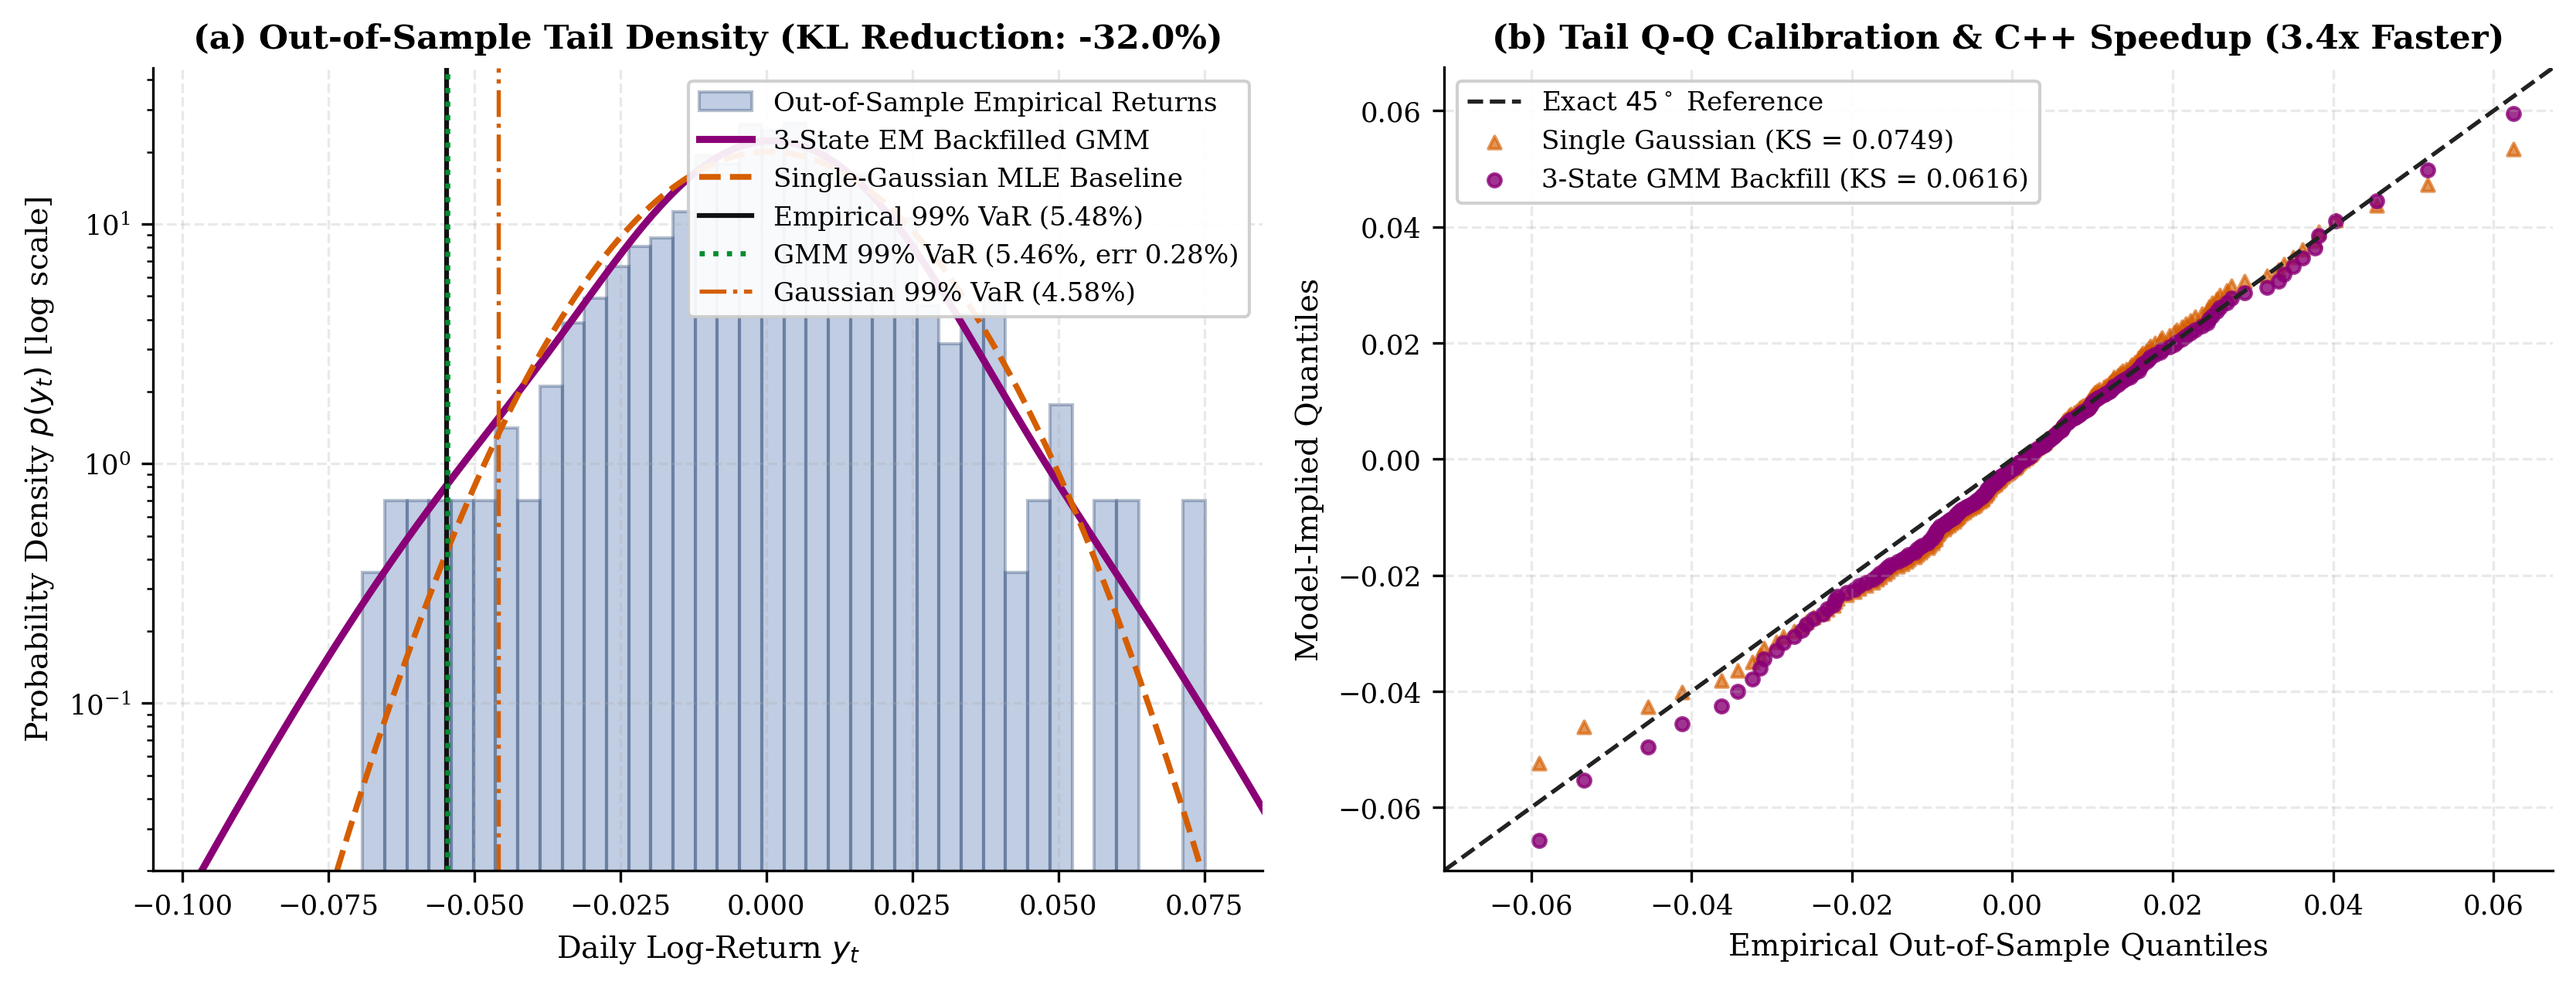
\includegraphics[width=0.96\textwidth]{../figures/fig1_gmm_qq_and_tail_var.png}\\[4pt]
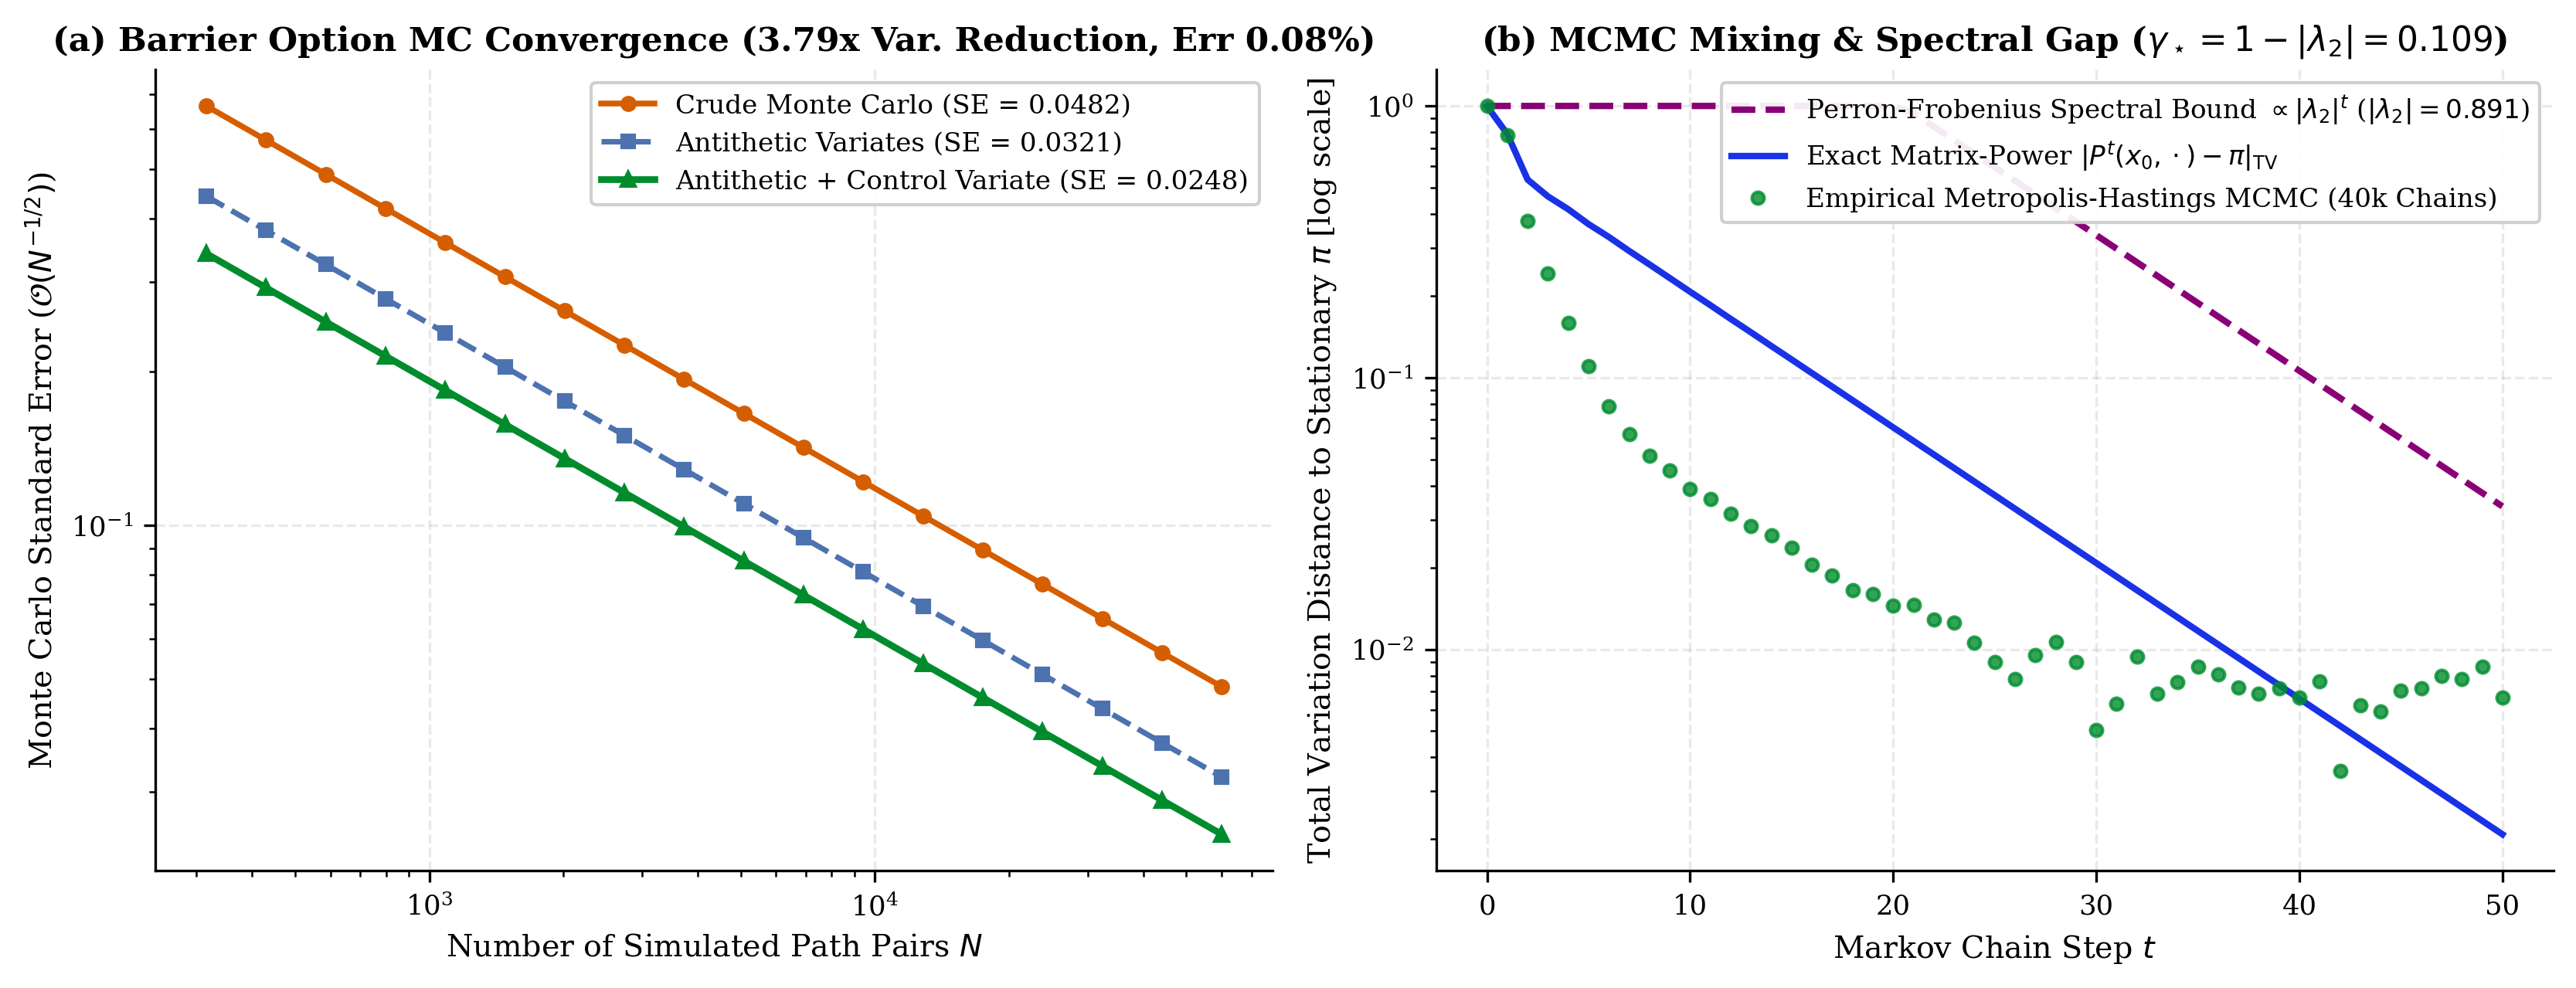
\includegraphics[width=0.96\textwidth]{../figures/fig2_mc_variance_reduction_convergence.png}\\[4pt]
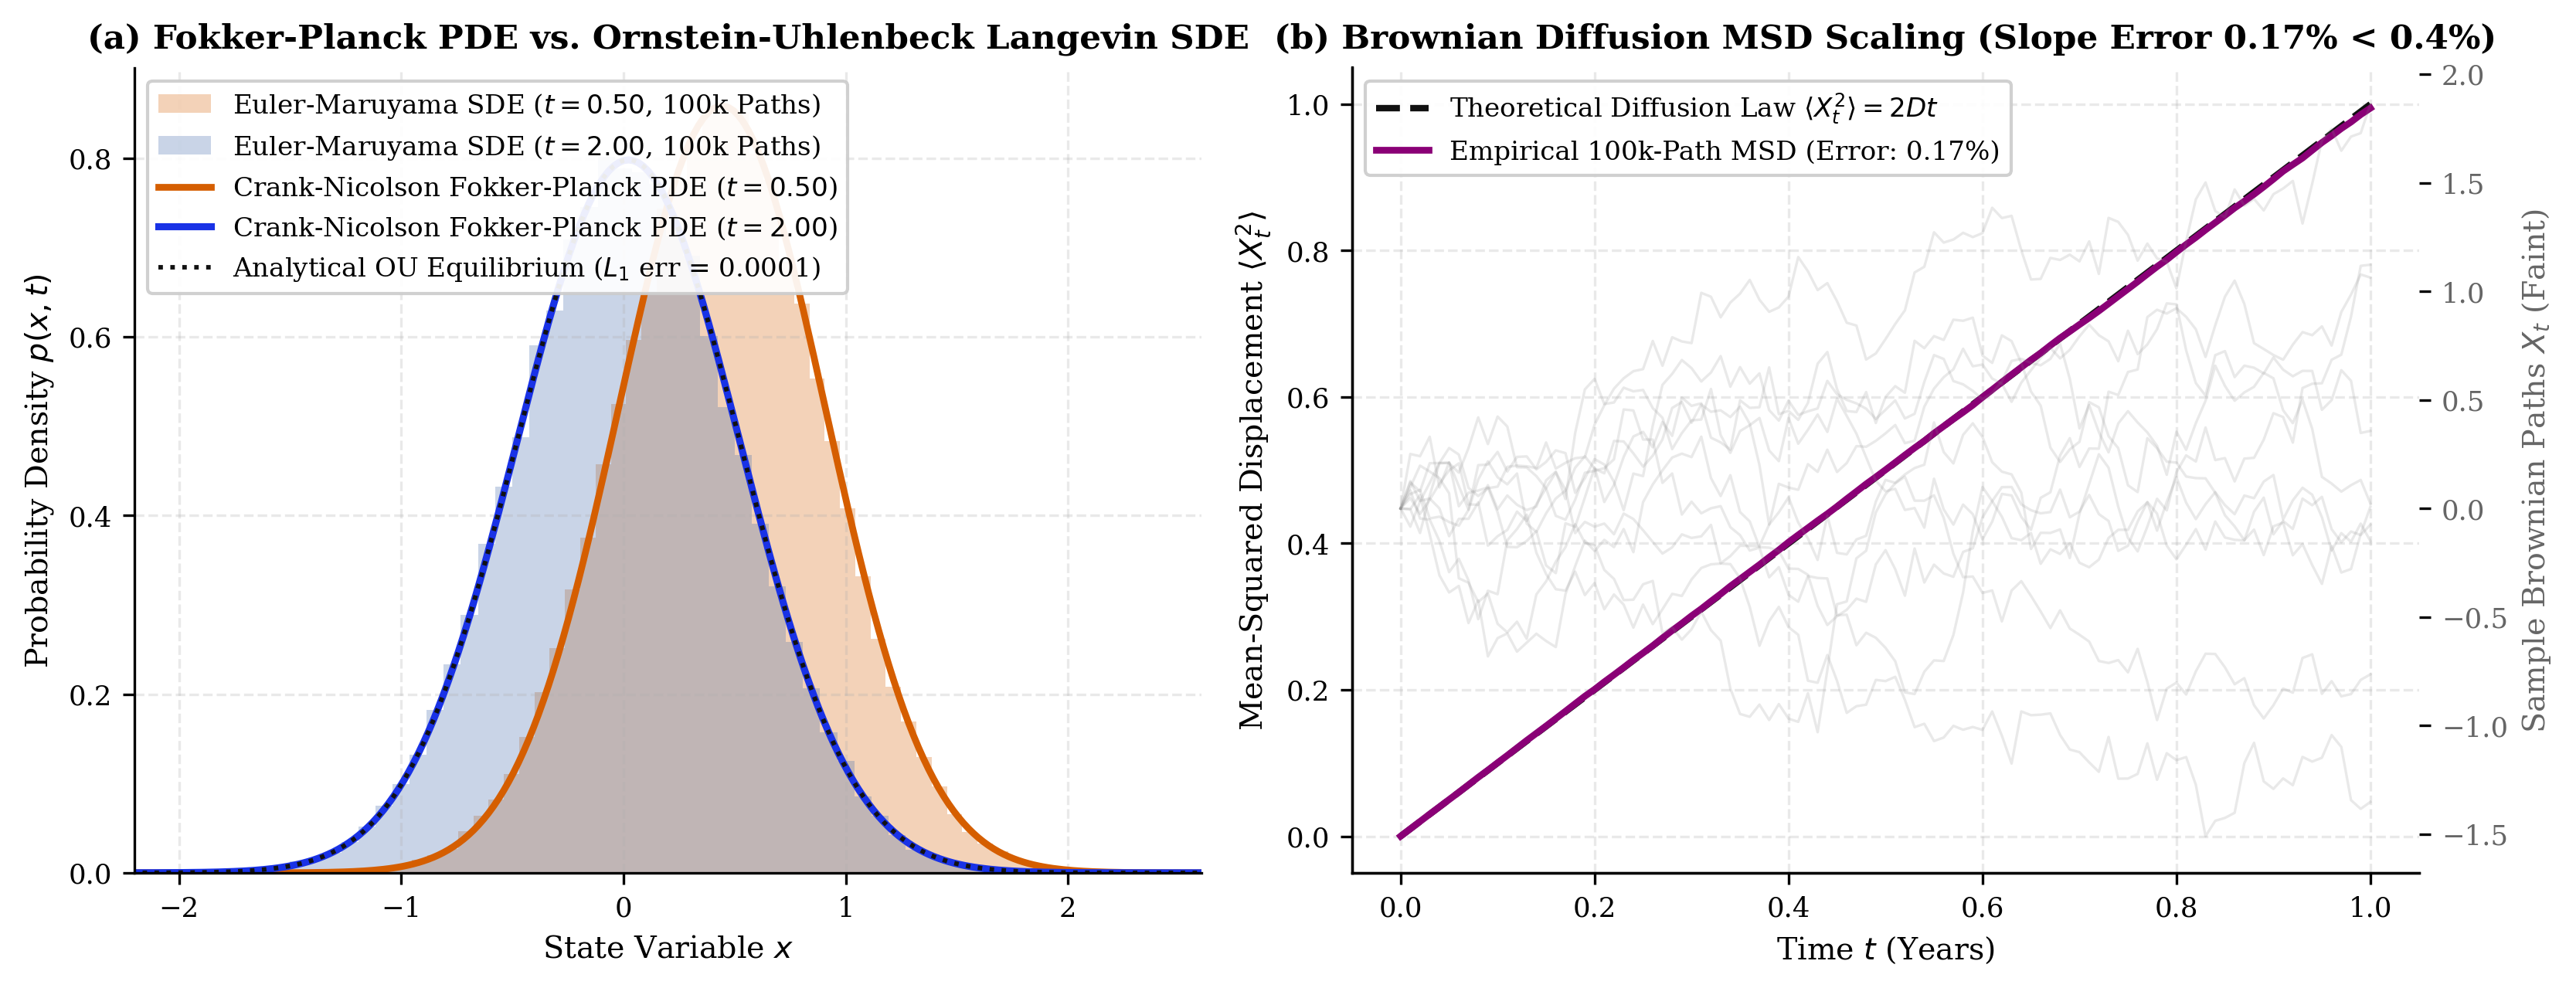
\includegraphics[width=0.96\textwidth]{../figures/fig3_fokker_planck_density_and_msd.png}
\caption{Top: Out-of-sample tail density, 99\% VaR backfilling, and Q--Q calibration for the 3-state GMM vs.\ single Gaussian. Middle: Monte Carlo standard error convergence ($\mathcal{O}(N^{-1/2})$) with antithetic + control variates, and Metropolis--Hastings TV convergence bounded by the Perron--Frobenius second eigenvalue $|\lambda_2|^t$. Bottom: Crank--Nicolson Fokker--Planck PDE vs.\ $10^5$-path Euler--Maruyama Ornstein--Uhlenbeck density and linear scaling of Brownian MSD $\langle X_t^2\rangle = 2Dt$.}
\end{figure*}

\end{document}

